\documentclass[10pt,twocolumn,letterpaper]{article}

\usepackage{cvpr}
\usepackage{times}
\usepackage{epsfig}
\usepackage{graphicx}
\usepackage{amsmath}
\usepackage{amssymb}

% Include other packages here, before hyperref.

% If you comment hyperref and then uncomment it, you should delete
% egpaper.aux before re-running latex.  (Or just hit 'q' on the first latex
% run, let it finish, and you should be clear).
\usepackage[breaklinks=true,bookmarks=false]{hyperref}

\cvprfinalcopy % *** Uncomment this line for the final submission

\def\cvprPaperID{****} % *** Enter the CVPR Paper ID here
\def\httilde{\mbox{\tt\raisebox{-.5ex}{\symbol{126}}}}

% Pages are numbered in submission mode, and unnumbered in camera-ready
%\ifcvprfinal\pagestyle{empty}\fi
\setcounter{page}{1}
\begin{document}

%%%%%%%%% TITLE
\title{Project proposal}

\author{Gunhee Lee, Jacob Morton\\
20172811, 20172327\\
Computer Science and Engineering, POSTECH\\
{\tt\small victorleee@postech.ac.kr}
}


\maketitle
%\thispagestyle{empty}


%%%%%%%%% BODY TEXT
\section{Abstract}

 We propose a Tell Generative Adversarial Network (TellGAN) which, given a face image with text in natural language, will generate plausible video frames of the given face speaking the given words. We call it TellGAN, because we tell the given face what to say. Although our project is related to lip reading, a well researched area, it appears that our text-to-video approach is the first of its kind. Our approach is devided into two parts, landmark trajectory prediction from a given word and generating a face and video frames from the predicted landmarks and initial face. We also propose a novel use of an LSTM to predict motion over a various number of frames. Among the several datasets used for lip reading, we used the GRID Corpus\footnote{http://spandh.dcs.shef.ac.uk/gridcorpus/}.
 
%------------------------------------------------------------------------
\section{Introduction}
 Text-Driven animation is not a new topic, but the known approaches use text-to-speech generators to drive animation and also do not use Deep Neural Networks (DNN) or Generative adversarial networks (GAN) for driving animation. Text-to-speech techniques offer some advantages, as it is easier to map continuous wave forms than discrete words to the continuous motions of the mouth during speech. Our proposed method will skip the text-to-speech generation by training a GAN and LSTMs with the aid of lip-reading techniques. Visual only lip reading is a heavily research topic and is essentially a Video-to-text problem. Our proposed approach is essentially the inverse to lip reading, a Text-to-Video problem.

 Generative adversarial networks has been improved in recent years. There also has been research which relates generative adversarial network and natural language processing. The text-to-image generation is one of the most obvious examples of it. 
  
 Our approach will also try to make an image from text in natural language. Compared with the normal image generation model, our model receives the input image. The contemporary state of the art network called AttentionGAN (Tao Xu et al.) can only change the image as a whole to meet the sentence direction, which is not desirable. For example, the minor changes that occure between frames would result in a completely different image. Our model would make the image more controllable than the previous approach. Also our model has a temporal component, as we propose generating a series of images that correspond spoken motions derived from the given input to make a video sequence. This has several challenges, among of which are maintaining temporal coherency and preventing errors cascading through future generated frames. Previous work on text-to-video using GAN exists\footnote{Video Generation From Text (Li, 2017)}. We will not use this method, as we will not have an end frame nor do we wish to use simultaneous generation of frame sequences. Instead we will opt for simplicity with a sequential approach that trends to more traditional text-to-image generation. 


%------------------------------------------------------------------------
\section{Dataset}
Since our approach is related to lip-reading, we can use many of the available datasets. We will choose to use the GRID Coprus. The dataset contains 33 individuals each speaking 1000 sentences. Each sentence is composed of 6 words. Video, audio, and timestamped transcripts (word level) are included. The recorded subjects are static in position, uniformly lit, with no expression. Instead of using a large vocabulary range (51 words), GRID tries cover more phonemes instead\footnote{An audio-visual corpus for speech perception and automatic speech recognition (Cooke, 2006)}. The smallest unit of speach is the phoneme. A word can easily converted into a set of phonemes. A viseme is the visual component  of the phoneme, where there is a many to one phoneme-to-viseme mapping. The english language is comprised of 45 phonemes which are mapped to 17 visemes according to the Fisher phoneme-to-viseme mapping\footnote{Confusions among visually perceived consonants (Fisher, 1968)}.


%------------------------------------------------------------------------
\section{Network Architecture}
 Our network is shown in Figure 1. The basic network architecture is a combination of two different networks. This network is a combination of Geometry-Contrastive GAN network(Qiao et al, arXiv, 2018) and Segmentation from Natural Language Expressions network(Hu et al, ECCV, 2016).
\begin{figure*}
\begin{center}
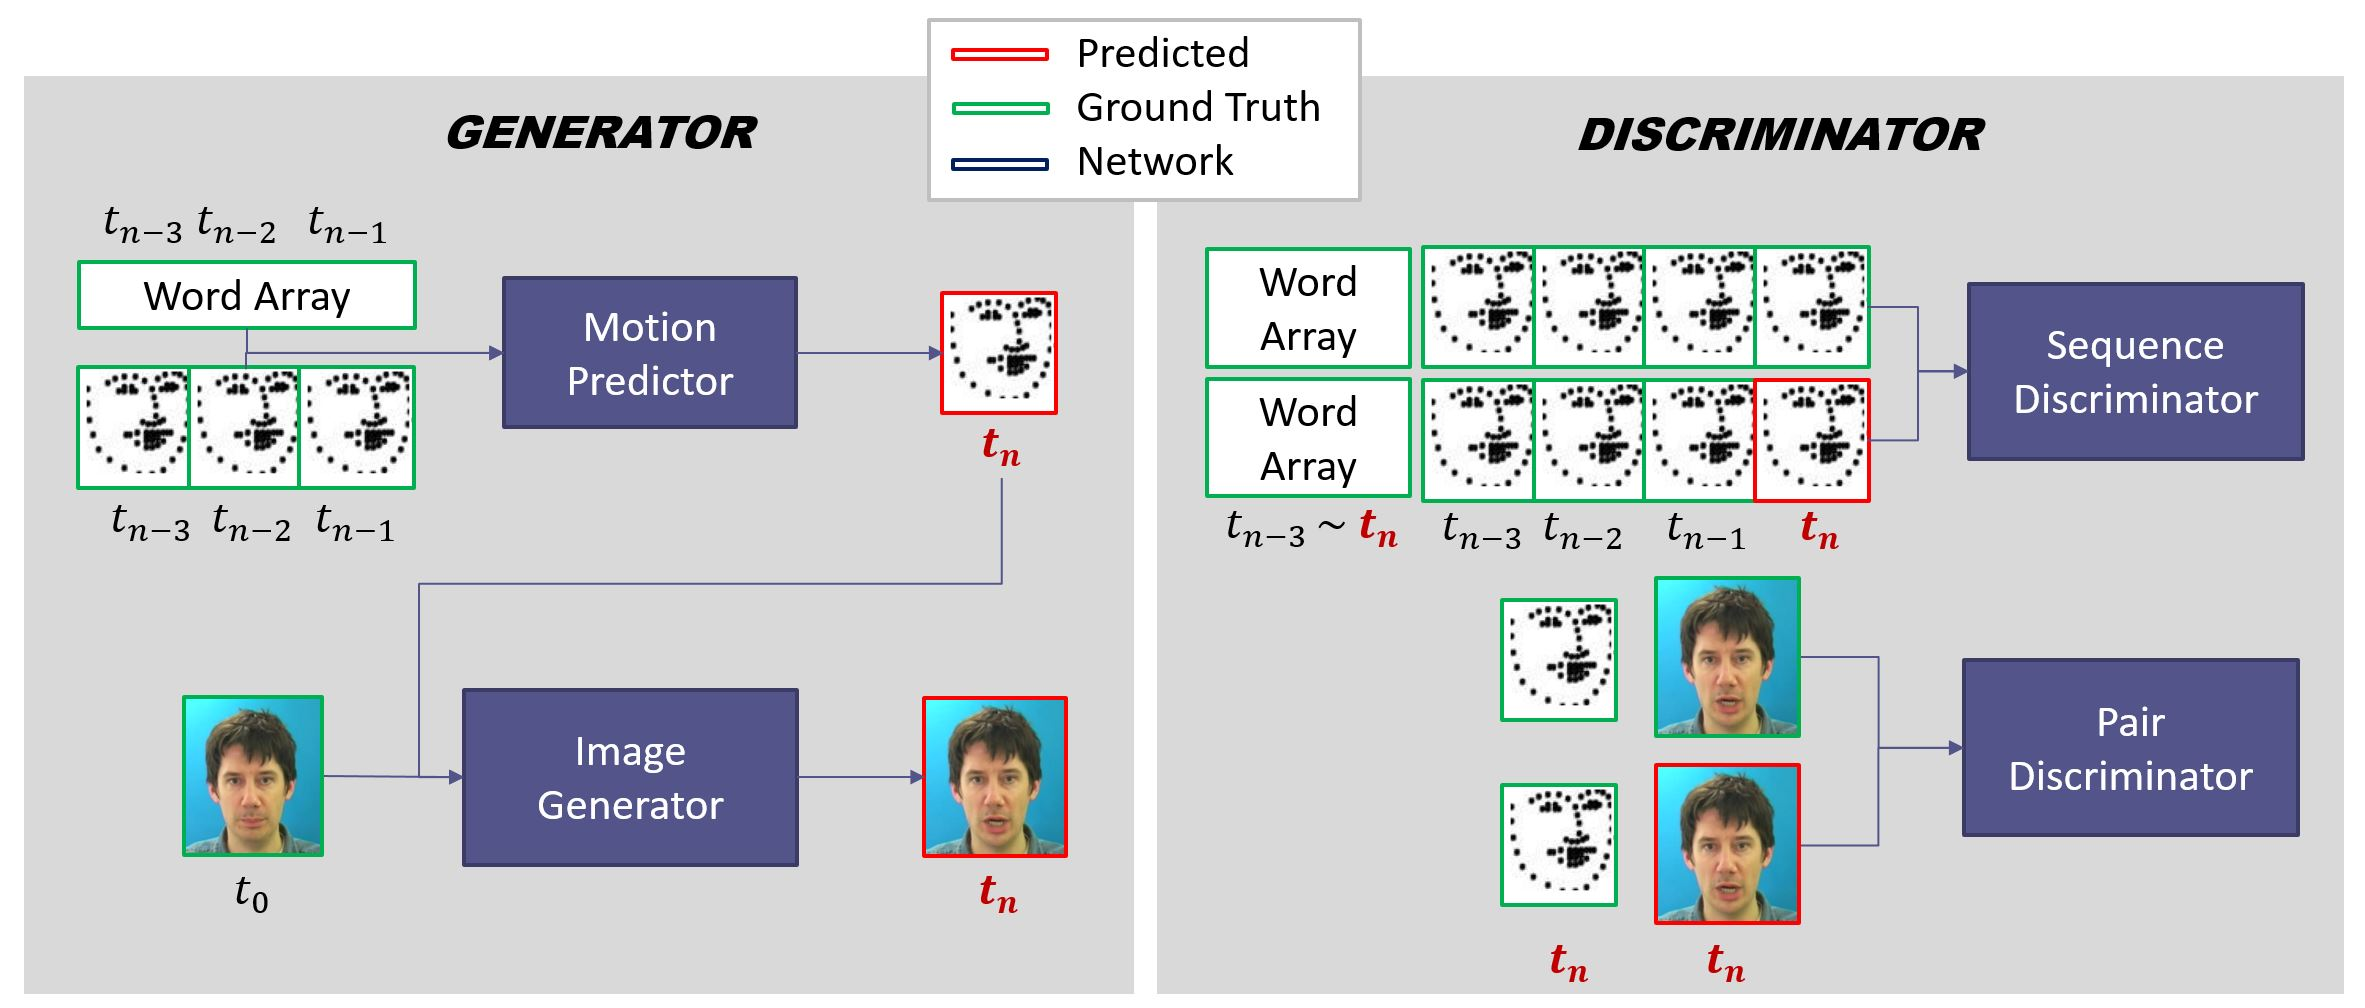
\includegraphics [scale=0.3] {images/network.JPG}
\end{center}
  \caption{The whole flow of our network. }
\label{fig:short}
\end{figure*}

For training, the natural sentence would be made directly by the label from paired data. The form of the sentence given to change the input image is limited. Something like ‘Change the color of the person to yellow’ or  ‘Rotate the head 40 degrees clockwise’ would be the most obvious example of the sentence.

The natural language is tokenized and changed into a word vector through a word embedding matrix. Then we use Long-Short Term Memory (LSTM) network to encode sequence data. At the end of the text sequence, we use the hidden state as the final encoded vector representation of the sentence.

On the other hand, the input image goes into the encoder part of the generator. This module can be a VGG type, ResNet type, or any other network. After it passes through the encoder part, the output is now turned into a high-level abstract feature. This feature is merged with the encoded expression from the natural language. Similar to the merging mechanism proposed in Hu et al, we concatenate the final encoded vector representation to the abstract feature at each location.

After the visual and language information is merged, the generator now up-samples the image. The upsampling network is not fixed yet. The decoder part will make the fake image from the input image.

 Now, The discriminator network discriminates the generator's fake images from the real image. The real image contains the target pose and color values. So that discriminator network is only given the image as an input. The discriminator computes the adversarial loss. Here we added another loss, the identity loss. The fake image should look almost like a real image which has the correct pose or color information. 

There are more things to improve with this network. This network can be improved using the region proposal network (RPN). This would select what and where to be changed. Affine transformation in the feature level could be added to the generator. This transformation module could help this image to be rotated (roll), scaled, and translated. The modification power would improve further if we improve this network.


{\small
\bibliographystyle{ieee}
\bibliography{egbib}
}

\end{document}




